% ─────────────────────────────────────────────────────────────────────────────
%
% Documentación del módulo de odometría visual-inercial (nav_odometry).
% Corresponde a la cuarta iteración del sistema de percepción local.
% ─────────────────────────────────────────────────────────────────────────────

\section{Odometría visual-inercial}
\label{sec:lm-vio}

Las tres iteraciones anteriores del módulo de percepción local establecieron
un pipeline capaz de proyectar la imagen de profundidad a una nube de puntos
3D, alinear esa nube a la dirección de la gravedad y ajustar el plano del
suelo mediante RANSAC jerárquico. Sin embargo, todos esos cálculos se realizan
en el marco instantáneo de la cámara: no existe ningún mecanismo que registre
el desplazamiento del usuario entre fotogramas consecutivos. La cuarta
iteración introduce el paquete \texttt{nav\_odometry}, un nodo independiente
de estimación de odometría visual-inercial (VIO, del inglés
\emph{Visual-Inertial Odometry}), cuyo resultado puede ser consumido por
módulos de acumulación de mapa y navegación.

\subsection{Marco teórico}
\subsubsection{Evolución de la orientación con cuaterniones}

Para describir la orientación de un cuerpo rígido en el espacio se utiliza el cuaternión unitario $\mathbf{q}(t)$, que representa la rotación desde el marco del cuerpo al marco del mundo. Sea $\mathbf{v}_{\text{body}}$ un vector fijo en el cuerpo. Su representación en el marco del mundo puede expresarse mediante:
%
\begin{equation}
    [0,\mathbf{v}_{\text{world}}]
    =
    \mathbf{q}(t)\otimes
    [0,\mathbf{v}_{\text{body}}]\otimes
    \mathbf{q}^*(t)
\end{equation}
%
donde $[0,\mathbf{v}]$ representa el cuaternión puro asociado al vector $\mathbf{v}$ y $\otimes$ denota el producto de Hamilton.
%
Utilizando que:
%
\begin{equation*}
    [0,\mathbf{v}_{body}]
    =
    \mathbf{q}^*\otimes
    [0,\mathbf{v}_{\text{world}}]\otimes
    \mathbf{q}
\end{equation*}
%
simplificando a $\mathbf{v}_{body}=\mathbf{v}$, la derivada puede reescribirse como:
%
\begin{equation*}
\begin{aligned}
    [0,\dot{\mathbf{v}}]
    &=
    \dot{\mathbf{q}}\otimes
    \mathbf{q}^*\otimes
    [0,\mathbf{v}]
    +
    [0,\mathbf{v}]\otimes
    \mathbf{q}\otimes
    \dot{\mathbf{q}}^*
\end{aligned}
\end{equation*}
%
Dado que el cuaternión es unitario:
%
\begin{equation*}
    \mathbf{q}\otimes\mathbf{q}^* = 1
\end{equation*}
%
su derivada satisface:
%
\begin{equation*}
    \dot{\mathbf{q}}\otimes
    \mathbf{q}^*
    +
    \mathbf{q}\otimes
    \dot{\mathbf{q}}^*
    =
    0
\end{equation*}
%
y por lo tanto:
%
\begin{equation*}
    \mathbf{q}\otimes
    \dot{\mathbf{q}}^*
    =
    -
    \dot{\mathbf{q}}\otimes
    \mathbf{q}^*
\end{equation*}
%
Reemplazando en la ecuación anterior:
%
\begin{equation*}
\begin{aligned}
    [0,\dot{\mathbf{v}}]
    &=
    \left(
        \dot{\mathbf{q}}\otimes
        \mathbf{q}^*
    \right)\otimes
    [0,\mathbf{v}]
    -
    [0,\mathbf{v}]\otimes
    \left(
        \dot{\mathbf{q}}\otimes
        \mathbf{q}^*
    \right)
\end{aligned}
\end{equation*}
%
Definiendo:
%
\begin{equation*}
    [0,\boldsymbol{\omega}_{\text{world}}]
    =
    2
    \dot{\mathbf{q}}\otimes
    \mathbf{q}^*
\end{equation*}
%
se obtiene:
%
\begin{equation*}
\begin{aligned}
    [0,\dot{\mathbf{v}}]
    =
    \frac{1}{2}
    \left(
        [0,\boldsymbol{\omega}]\otimes
        [0,\mathbf{v}]
        -
        [0,\mathbf{v}]\otimes
        [0,\boldsymbol{\omega}]
    \right)
\end{aligned}
\end{equation*}
%
Usando la propiedad del producto entre cuaterniones puros:
%
\begin{equation*}
    [0,\mathbf{a}] \otimes
    [0,\mathbf{b}]
    -
    [0,\mathbf{b}]\otimes
    [0,\mathbf{a}]
    =
    [0,2(\mathbf{a}\times\mathbf{b})]
\end{equation*}
%
resulta:
%
\begin{equation*}
    [0,\dot{\mathbf{v}}]
    =
    [0,\boldsymbol{\omega}\times\mathbf{v}]
\end{equation*}%
lo cual coincide con la ecuación cinemática rotacional clásica.
\begin{equation}
    \label{eq:rotacional-clasica}
    \dot{\mathbf{v}} = \boldsymbol{\omega}\times\mathbf{v}
\end{equation}
%

Finalmente, a partir de:
%
\begin{equation*}
    [0,\boldsymbol{\omega}_{\text{world}}]
    =
    2
    \dot{\mathbf{q}}\otimes
    \mathbf{q}^*
\end{equation*}
%
y multiplicando a derecha por $\mathbf{q}$:
%
\begin{equation*}
\begin{aligned}
    [0,\boldsymbol{\omega}_{\text{world}}]\otimes
    \mathbf{q}
    &=
    2
    \dot{\mathbf{q}}\otimes
    \mathbf{q}^*\otimes
    \mathbf{q}
    =
    2\dot{\mathbf{q}}
\end{aligned}
\end{equation*}
%
se obtiene:
%
\begin{equation*}
    \dot{\mathbf{q}}
    =
    \frac{1}{2}
    [0,\boldsymbol{\omega}_{\text{world}}]\otimes
    \mathbf{q}
\end{equation*}
%
Si la velocidad angular se expresa en el marco del cuerpo:
%
\begin{equation*}
    [0,\boldsymbol{\omega}_{\text{world}}]
    =
    \mathbf{q}\otimes
    [0,\boldsymbol{\omega}_{\text{body}}]\otimes
    \mathbf{q}^*
\end{equation*}
%
entonces:
%
\begin{equation}
\begin{aligned}
    \dot{\mathbf{q}}
    &=
    \frac{1}{2}
    \mathbf{q}\otimes
    [0,\boldsymbol{\omega}_{\text{body}}]
    \label{eq:dot_q}
\end{aligned}
\end{equation}
%
que corresponde a la ecuación diferencial utilizada habitualmente en navegación inercial y filtros de actitud.

\subsubsection{Naturaleza del drift en sistemas inerciales}

Una unidad de medición inercial (IMU, del inglés
\emph{Inertial Measurement Unit}) estima el movimiento integrando la
velocidad angular reportada por el giroscopio. La orientación se obtiene
integrando:
%
\begin{equation}
  \label{eq:gyro-integration}
  \dot{\mathbf{q}}(t) = \tfrac{1}{2}\,\mathbf{q}(t) \otimes
  \begin{bmatrix}0 \\ \boldsymbol{\omega}(t)\end{bmatrix}
\end{equation}
%
donde $\mathbf{q} \in \mathbb{H}_1$ es el cuaternión unitario que representa
la rotación del marco del cuerpo al marco de referencia y $\otimes$ denota el
producto de Hamilton \cite{Woodman2007}.

El error de integración crece con el tiempo por dos causas principales
\cite{Woodman2007}: el ruido de densidad espectral del giroscopio
($\sigma_g \approx 1{,}6 \times 10^{-4}\,\text{rad/s}/\!\sqrt{\text{Hz}}$
para el D435i \cite{RS-D400}) y el drift de bias, un offset sistemático
lentamente variable que hace al sensor reportar velocidad angular no nula en
reposo. El resultado es una deriva de orientación que afecta especialmente al
yaw, el ángulo de rotación alrededor del eje vertical.

\subsubsection{Por qué el acelerómetro no resuelve el yaw}

A diferencia del pitch y el roll, que pueden corregirse mediante el vector de
gravedad medido por el acelerómetro, el yaw carece de referencia absoluta sin
magnetómetro o fuente externa. El acelerómetro mide la aceleración específica:
%
\begin{equation}
  \label{eq:accel-model}
  \mathbf{a}_{\text{meas}} = \mathbf{R}^{T}(\mathbf{a}_{\text{real}} - \mathbf{g})
\end{equation}
%
donde $\mathbf{R}$ es la matriz de rotación del cuerpo al mundo y $\mathbf{g}$
es el vector de gravedad en el marco del mundo. En reposo
$\mathbf{a}_{\text{real}} = \mathbf{0}$, de modo que
$\mathbf{a}_{\text{meas}} = -\mathbf{R}^{T}\mathbf{g}$.

La gravedad define una dirección en el espacio tridimensional, no un punto.
Conocer esa dirección en el marco del cuerpo determina únicamente pitch y
roll, pero deja libre el ángulo de rotación alrededor del eje vertical.
Formalmente, la transformación $\mathbf{R} \to \mathbf{R}\,\mathbf{R}_{\psi}$,
para cualquier rotación $\mathbf{R}_{\psi}$ alrededor del eje vertical, deja
$\mathbf{a}_{\text{meas}}$ invariante \cite{Hartley2004}. En el sistema aquí
descrito el magnetómetro no es viable por interferencia electromagnética de los
motores vibradores que componen la matriz háptica, por lo que la corrección de
yaw debe provenir de la visión.

\subsubsection{Filtro complementario de Mahony}

El filtro complementario propone combinar el giroscopio, que aporta alta
frecuencia y baja latencia, con la visión, que provee referencia a largo plazo
para la corrección del drift. La formulación de Mahony \cite{Madgwick2010}
plantea un regulador proporcional-integral en tiempo continuo que corrige el
giroscopio con el error observado en el marco del cuerpo:
%
\begin{equation}
  \label{eq:mahony-correction}
  \hat{\boldsymbol{\omega}}_{\text{corr}} =
  \boldsymbol{\omega} - \hat{\mathbf{b}} + K_p\,\mathbf{e} + K_i\!\int_0^t \mathbf{e}\,d\tau
\end{equation}
%
donde $\mathbf{e}$ es el vector de error en el marco del cuerpo,
$\hat{\mathbf{b}}$ es la estimación del bias, y $K_p$, $K_i$ son las ganancias
de realimentación. El cuaternión se actualiza integrando $\hat{\boldsymbol{\omega}}_{\text{corr}}$.

A partir de la ecuación~\ref{eq:dot_q} se puede aproximar, para $\delta t$ pequeño, por la expansión de Euler:
%
\begin{equation}
\label{eq:euler-linearization}
\mathbf{q}(t+\delta t) \approx \mathbf{q}(t) + \frac{1}{2}\,\mathbf{q}(t) \otimes [0,\,\boldsymbol{\omega}_c\,\delta t]
\end{equation}
%
Esta forma corresponde a la linearización de primer orden de la exponencial, y es equivalente a multiplicar por $dq \approx [1,\,\boldsymbol{\omega}_c\,\delta t/2]$. Sin embargo, esta aproximación no preserva la norma unitaria del cuaternión, por lo que en la práctica se prefiere la integración exponencial exacta (ecuación~\ref{eq:exp-map-explicit}), seguida de renormalización si es necesario.



El cuaternión se actualiza integrando
$\hat{\boldsymbol{\omega}}_{\text{corr}}$ mediante el mapa exponencial exacto
en $SO(3)$, evitando la pérdida de norma unitaria que produce la linearización
de Euler de primer orden:
%
\begin{equation}
  \label{eq:exp-map}
  \mathbf{q}(t+\delta t) =
  \mathbf{q}(t) \otimes \exp\!\left(\tfrac{1}{2}\,
  \hat{\boldsymbol{\omega}}_{\text{corr}}\,\delta t\right)
\end{equation}
%
La exponencial de un cuaternión puro $\tfrac{1}{2}\boldsymbol{\omega}_c\,\delta t$
se evalúa mediante la fórmula cerrada de eje-ángulo. Definiendo
$\theta = \|\boldsymbol{\omega}_c\,\delta t\|$ como el ángulo de rotación en el
intervalo $\delta t$, la expansión de la exponencial en la esfera unitaria
$\mathbb{H}_1$ es:
%
\begin{equation}
  \label{eq:exp-map-explicit}
  \exp\!\left(\tfrac{1}{2}\boldsymbol{\omega}_c\,\delta t\right)
  = \left[\cos\frac{\theta}{2},\;
          \frac{\sin(\theta/2)}{\theta}\,\boldsymbol{\omega}_c\,\delta t\right]
\end{equation}
%

Para ángulos pequeños ($\theta \ll 1$), la expansión de Taylor
$\cos(\theta/2) \approx 1$ y $\sin(\theta/2) \approx \theta/2$ reduce la
ecuación~\ref{eq:exp-map-explicit} a $dq \approx [1,\,\boldsymbol{\omega}_c\,\delta t/2]$,
que coincide con la linearización de Euler de primer orden. La implementación
en \texttt{fromOmegaDt()} evalúa siempre la forma exacta
(ecuación~\ref{eq:exp-map-explicit}), recurriendo a la identidad
$\mathbf{q} \leftarrow \mathbf{q}(t) \otimes dq$ seguida de
renormalización explícita.

Para el acelerómetro el vector de error es el producto vectorial entre la
medición normalizada y la dirección esperada de la gravedad transformada al
marco del cuerpo:
%
\begin{equation}
  \label{eq:accel-error}
  \mathbf{e}_a =
  \hat{\mathbf{a}}_{\text{meas}} \times
  \left(\mathbf{q}^{-1} \cdot \hat{\mathbf{g}}_{\text{world}}\right)
\end{equation}
%
donde $\hat{\mathbf{g}}_{\text{world}} = (0,\,1,\,0)^T$ (convención Y abajo,
coherente con el resto del pipeline). El producto vectorial en la
ecuación~\ref{eq:accel-error} proporciona el eje de rotación necesario para
alinear la estimación con la medición.

Para el yaw, cuando el módulo de odometría visual entrega una rotación relativa
$\Delta\mathbf{R}_{\text{vis}}$ con confianza $r \in [0,1]$, se computa el
error entre la estimación del giroscopio y la visual, y se aplica una
corrección proporcional alrededor del eje vertical del mundo:
%
\begin{equation}
  \label{eq:yaw-correction}
  \Delta\mathbf{q}_{\text{yaw}} =
  \text{fromAngleAxis}\!\left(\alpha_{\text{yaw}}\cdot r \cdot e_{\text{yaw}},\;
  \hat{\mathbf{y}}_{\text{world}}\right)
\end{equation}
%
donde $\alpha_{\text{yaw}} \in [0,1]$ es la ganancia de corrección configurable
y $e_{\text{yaw}}$ es la componente del error de orientación proyectada sobre
el eje vertical.

A modo de resumen, la Figura~\ref{fig:mahony-blockdiagram} muestra el diagrama
en bloques del filtro, donde se aprecia el lazo de realimentación
proporcional-integral sobre el error de inclinación y la conexión entre
el integrador exp-map y la estimación de orientación $\mathbf{q}$.

\begin{figure}[h]
  \centering
  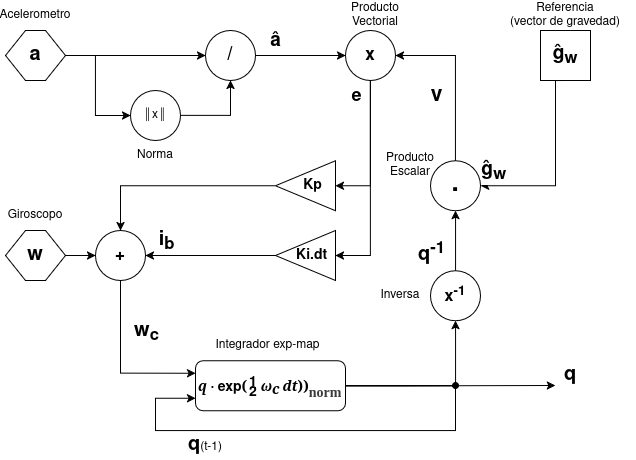
\includegraphics[width=0.55\textwidth]{_Imagenes/odom/mahony.drawio.png}
  \caption{Diagrama en bloques del filtro complementario de Mahony.
    Las entradas son la velocidad angular $\boldsymbol{\omega}$ del giroscopio
    y la aceleración $\mathbf{a}$ del acelerómetro. El lazo PI corrige el
    giroscopio con el error de inclinación $\mathbf{e}$; el integrador
    exp-map en $SO(3)$ produce la orientación $\mathbf{q}$, que se
    realimenta para calcular la gravedad esperada $\mathbf{v}$ en cada ciclo.}
  \label{fig:mahony-blockdiagram}
\end{figure}

La Tabla~\ref{tab:vio-mahony-steps} resume los seis pasos de cómputo que
ejecutael filtro en cada muestra de IMU, como referencia rápida de las
ecuaciones~\ref{eq:mahony-correction}--\ref{eq:accel-error}.

\begin{table}[h]
\centering
\caption{Pasos de cómputo del filtro de Mahony por muestra de IMU.}
\label{tab:vio-mahony-steps}
\begin{tabularx}{\textwidth}{llX}
\hline
\textbf{Paso} & \textbf{Variable} & \textbf{Operación} \\
\hline
Normalización del acelerómetro
  & $\hat{\mathbf{a}}$
  & $\hat{\mathbf{a}} = \mathbf{a}/\|\mathbf{a}\|$,\quad
    solo si $\|\mathbf{a}\| \in \bigl[g\cdot 0{,}7,\; g\cdot 1{,}3\bigr]$ \\[2pt]
Gravedad esperada en cuerpo
  & $\mathbf{v}$
  & $\mathbf{v} = \mathbf{q}^{-1} \cdot \hat{\mathbf{g}}_W$,\quad
    $\hat{\mathbf{g}}_W = (0,\,-1,\,0)^T$ \\[2pt]
Error de inclinación
  & $\mathbf{e}$
  & $\mathbf{e} = \hat{\mathbf{a}} \times \mathbf{v}$ \\[2pt]
Actualización del integrador
  & $\mathbf{i}_b$
  & $\mathbf{i}_b \mathrel{+}= \mathbf{e}\cdot K_i \cdot \delta t$ \\[2pt]
Corrección del giroscopio
  & $\boldsymbol{\omega}_c$
  & $\boldsymbol{\omega}_c = \boldsymbol{\omega} + \mathbf{e}\cdot K_p + \mathbf{i}_b$ \\[2pt]
Integración del cuaternión (exp-map $SO(3)$)
  & $\mathbf{q}$
  & $\mathbf{q} \leftarrow \bigl(\mathbf{q} \otimes
    \exp(\tfrac{1}{2}\,\boldsymbol{\omega}_c\,\delta t)\bigr)_{\!\text{norm}}$ \\[2pt]
\hline
\end{tabularx}
\end{table}

Para la corrección de yaw, la Tabla~\ref{tab:vio-yaw-correction} detalla los
pasos del método \texttt{applyVisualUpdate()}, cuyo resultado corresponde a
la ecuación~\ref{eq:yaw-correction}. El subíndice ``cap'' denota la
orientación capturada por el estimador justo antes de invocar el tracker
(variable \texttt{q\_at\_capture} en la implementación).

\begin{table}[h]
\centering
\caption{Pasos de la corrección de yaw por odometría visual.}
\label{tab:vio-yaw-correction}
\begin{tabularx}{\textwidth}{llX}
\hline
\textbf{Paso} & \textbf{Variable} & \textbf{Operación} \\
\hline
Orientación visual esperada
  & $\mathbf{q}_{\text{vis}}$
  & $\mathbf{q}_{\text{vis}} = \mathbf{q}_{\text{cap}} \otimes
    \Delta\mathbf{R}_{\text{body}}$ \\[2pt]
Error en marco del cuerpo
  & $\Delta\mathbf{R}_{\text{err}}$
  & $\Delta\mathbf{R}_{\text{err}} = \mathbf{q}^{-1} \otimes
    \mathbf{q}_{\text{vis}}$ \\[2pt]
Error en marco del mundo
  & $\Delta\mathbf{R}_{\text{err}}^W$
  & $\Delta\mathbf{R}_{\text{err}}^W = \mathbf{q} \otimes
    \Delta\mathbf{R}_{\text{err}} \otimes \mathbf{q}^{-1}$ \\[2pt]
Componente de yaw (ángulo pequeño)
  & $e_\psi$
  & $e_\psi \approx 2 \cdot \Delta R^W_{\text{err},y}$ \\[2pt]
Corrección aplicada al cuaternión
  & $\mathbf{q}$
  & $\mathbf{q} \leftarrow
    \text{fromAngleAxis}(\alpha_{\text{yaw}} \cdot r \cdot e_\psi,\;
    \hat{\mathbf{y}}_W) \otimes \mathbf{q}$ \\[2pt]
\hline
\end{tabularx}
\end{table}

\subsubsection{Comparación de enfoques VIO}

Existen tres líneas principales de trabajo para la fusión visual-inercial
\cite{Forster2017}:

\begin{description}
  \item[Acoplamiento ajustado (\emph{tightly coupled}).] La IMU y la visión
    comparten el mismo estado en un grafo de factores o en un filtro de Kalman
    de estados múltiples (MSCKF \cite{Mourikis2007}). Ejemplos: OpenVINS y
    VINS-Mono \cite{Qin2018}. Ofrece mayor robustez ante pérdida visual, pero
    su integración es más compleja.

  \item[Acoplamiento suelto (\emph{loosely coupled}).] La odometría visual se
    estima de forma independiente y luego se fusiona con la IMU mediante un
    segundo filtro. Es el enfoque aquí implementado. Resulta más modular y
    sencillo de depurar, a cambio de perder información marginal entre ambas
    fuentes.

  \item[Filtros frente a optimización.] Los filtros (EKF, complementario)
    operan en tiempo real con complejidad constante por fotograma. Los métodos
    de optimización (grafo de factores, bundle adjustment) permiten refinar la
    trayectoria con mayor precisión, pero no son adecuados para tiempo real en
    hardware embebido \cite{Engel2018}.
\end{description}

Para este sistema se seleccionó el acoplamiento suelto con filtro
complementario de Mahony como solución mínima viable por las siguientes
razones: (a)~permite intercambiar el backend visual sin modificar el pipeline
de fusión, gracias a la interfaz abstracta \texttt{IOdometryBackend};
(b)~tiene complejidad $O(1)$ por muestra de IMU, compatible con la Raspberry
Pi~5 \cite{RaspberryPi}; (c)~la literatura reporta resultados satisfactorios
con enfoques similares en aplicaciones peatonales portátiles
\cite{Lee2016RGBD, Zhang2021DVIO}.

\subsection{Arquitectura del módulo}

El paquete \texttt{nav\_odometry} implementa una arquitectura desacoplada en
seis capas. La Tabla~\ref{tab:vio-capas} resume cada componente, su función
y sus dependencias externas.

\begin{table}[h]
\centering
\caption{Capas del paquete \texttt{nav\_odometry}.}
\label{tab:vio-capas}
\begin{tabularx}{\textwidth}{lXl}
\hline
\textbf{Componente} & \textbf{Función} & \textbf{Dependencias} \\
\hline
\texttt{nav\_math} & Tipos y álgebra matemática (compartido con \texttt{local\_mapper}) & C++17 puro \\
\texttt{IOdometryBackend} & Interfaz intercambiable de backend & C++17 puro \\
\texttt{ComplementaryFilter} & Filtro de Mahony (fusión IMU + visión) & C++17 puro \\
\texttt{RgbdTracker} & Odometría visual LK + PnP con profundidad de hardware & OpenCV 4 \\
\texttt{OdometryEstimator} & Backend concreto (orquestador) & Todas las anteriores \\
\texttt{OdometryNode} & Nodo ROS~2 & ROS~2, cv\_bridge \\
\hline
\end{tabularx}
\end{table}

\subsubsection{Paquete compartido de tipos matemáticos (\texttt{nav\_math})}

Dado que \texttt{nav\_odometry} y \texttt{local\_mapper} operan sobre
representaciones geométricas comunes, se optó por centralizar estas
abstracciones en un paquete independiente denominado \texttt{nav\_math}.
El paquete expone el archivo \texttt{types.hpp}, que define los tipos
fundamentales del pipeline: \texttt{Vec3}, \texttt{Quaternion},
\texttt{Pose}, \texttt{OdometryState}, \texttt{ImuSample}, \texttt{ColorFrame}
y \texttt{CameraIntrinsics}. No tiene dependencias en ROS~2 ni en OpenCV.
La convención de coordenadas interna, Y apuntando hacia abajo en la dirección
de la gravedad, es coherente con el resto del pipeline iniciado en la V1 del
módulo.

\subsubsection{Interfaz de backend (\texttt{IOdometryBackend})}

La clase abstracta \texttt{IOdometryBackend} declara la API que cualquier
backend debe implementar:
\begin{itemize}
  \item \texttt{processImu()}: acepta una muestra de IMU a alta frecuencia.
  \item \texttt{processRgbd()}: acepta un frame de color con su mapa de
    profundidad asociado.
  \item \texttt{getState()}: consulta el estado de odometría de forma
    segura para hilos (\emph{thread-safe}).
  \item \texttt{setCameraIntrinsics()}: configura los parámetros de la cámara.
\end{itemize}

Esta interfaz permite, por ejemplo, reemplazar el backend por el MSCKF de
OpenVINS \cite{Mourikis2007} o por ORB-SLAM3 \cite{Mur2015ORB} modificando
únicamente el punto de construcción en \texttt{OdometryNode}, sin alterar
el resto del pipeline.

\subsubsection{Filtro complementario (\texttt{ComplementaryFilter})}

Implementa el filtro de Mahony descrito en las
ecuaciones~\ref{eq:mahony-correction}--\ref{eq:yaw-correction} del marco
teórico. Los parámetros configurables son:
\begin{itemize}
  \item $K_p = 2{,}0$: ganancia proporcional de realimentación del
    acelerómetro.
  \item $K_i = 0{,}005$: ganancia integral para eliminar el offset DC.
  \item $\alpha_{\text{yaw}} = 0{,}1$: fracción de corrección de yaw aplicada
    por cada actualización visual.
  \item Tolerancia de módulo de $g$: acepta mediciones del acelerómetro
    dentro de $\pm 30\,$\% de $9{,}807\,\text{m/s}^2$, descartando
    aceleraciones lineales bruscas que corrompan la referencia de gravedad.
\end{itemize}

La integración del cuaternión emplea el mapa exponencial exacto
(ecuación~\ref{eq:exp-map}), que preserva la norma unitaria bajo integración
discreta a diferencia de la actualización de Euler de primer orden.

Adicionalmente, el método \texttt{applyVisualUpdate()} aplica una corrección
débil de roll y pitch mediante interpolación esférica (\emph{slerp}) con
ganancia $\alpha_{\text{yaw}} \cdot 0{,}1 \cdot r$ hacia la orientación visual
completa. Esta corrección complementa la ya existente del acelerómetro: en
movimiento activo, el acelerómetro confunde aceleración lineal con gravedad,
mientras que la visión proporciona una referencia de orientación independiente.

\subsection{Método}
\label{sec:lm-vio-metodo}

El algoritmo de odometría visual propuesto se implementa en dos componentes
principales: el \texttt{RgbdTracker}, que estima la pose relativa entre
fotogramas mediante flujo óptico y profundidad de hardware, y el
\texttt{OdometryEstimator}, que integra esa estimación con el filtro de
Mahony y publica el estado fusionado.

\subsubsection{Tracker RGBD (\texttt{RgbdTracker})}

El \texttt{RgbdTracker} estima la pose relativa entre fotogramas consecutivos
combinando flujo óptico con profundidad de hardware. El pipeline se divide en
cinco etapas que se detallan a continuación.

La imagen utilizada como entrada al tracker es la imagen a color del D435i,
convertida a escala de grises. Una alternativa natural sería emplear
la cámara infrarroja integrada del sensor, cuya ausencia de crominancia
simplificaría el pipeline. Sin embargo, el D435i proyecta sobre la escena un
patrón estructurado de puntos infrarrojos para mejorar la estimación de
profundidad en superficies poco texturadas. El detector FAST, basado en
contraste local de intensidad, clasifica estos puntos proyectados como
esquinas de alta respuesta: al ser fijos respecto al sensor y no respecto a la
escena, generan falsas correspondencias sistemáticas entre fotogramas
consecutivos que degradan la estimación de movimiento. Varios sistemas de
odometría y mapeo con cámaras RGB-D abordan este problema empleando la imagen
a color para la extracción de características visuales
\cite{Endres2014, sturm12iros}. Una alternativa reportada en la literatura
consiste en desactivar el emisor infrarrojo durante la captura visual,
opción que expone la imagen IR de los fotodetectores del sensor sin la
interferencia del patrón proyectado \cite{IntelRealSenseDepthTuning}; en el
sistema aquí descrito, sin embargo, esa opción no es viable, dado que la
imagen de profundidad se genera a partir precisamente de ese patrón infrarrojo
proyectado y constituye la fuente principal de información de los módulos
\texttt{local\_mapper} y \texttt{depth\_grid\_encoder}. La imagen a color,
alineada espacialmente con el mapa de profundidad mediante la calibración de
fábrica del sensor (\texttt{aligned\_depth\_to\_color}), provee
características visuales libres de esta interferencia.

\paragraph{Etapa 1: detección distribuida de esquinas FAST.}

El detector FAST (\emph{Features from Accelerated Segment Test})
\cite{Rosten2006FAST} clasifica un píxel $\mathbf{p}$ como esquina si existe
un arco contiguo de $n = 12$ píxeles sobre una circunferencia de radio 3
que sean todos más brillantes que $I(\mathbf{p}) + t$ o todos más oscuros
que $I(\mathbf{p}) - t$, donde $t$ es el umbral de respuesta. El parámetro
configurable \texttt{fast\_threshold} (valor por defecto: 20 unidades de
intensidad en escala de grises) controla la sensibilidad: valores bajos
detectan más esquinas pero aumentan la tasa de falsas detecciones en regiones
de baja textura.

Para evitar el agrupamiento espacial de características en zonas de alta
textura, la imagen se subdivide en una grilla de $4 \times 3$ celdas.
En cada celda se ejecuta FAST de forma independiente y se retienen las
$\lceil N_{\max} / 12 \rceil$ esquinas de mayor respuesta, donde
$N_{\max}$ es el número máximo total de puntos rastreados (valor por defecto:
\texttt{max\_features} $= 300$). Los puntos se ordenan por su puntuación de
respuesta de mayor a menor antes de recortar, garantizando que los más
discriminativos tengan prioridad dentro de cada celda.

\paragraph{Etapa 2: proyección a coordenadas 3D (\emph{depth lifting}).}

Antes de procesar la odometría, cada punto detectado en el fotograma de
referencia se eleva al espacio 3D utilizando el mapa de profundidad
\texttt{aligned\_depth\_to\_color} del D435i. La operación de
\emph{depth lifting} es la inversa de la proyección perspectiva del modelo
pinhole: dado el valor de profundidad $d$ en el píxel $(u, v)$, se recuperan
las coordenadas 3D en el marco de la cámara sin necesidad de triangulación
estereoscopíca. El modelo pinhole establece que estas coordenadas son:
%
\begin{equation}
  \label{eq:lifting}
  \mathbf{P} =
  \left(
    \frac{(u - c_x)\,d}{f_x},\;
    \frac{(v - c_y)\,d}{f_y},\;
    d
  \right)
\end{equation}
%
donde $d = z_{\text{raw}} \cdot s$ es la profundidad en metros con factor de
escala $s = 0{,}001$ para el D435i \cite{RS-D400}, y
$(f_x,\, f_y,\, c_x,\, c_y)$ son los parámetros intrínsecos de la cámara de
color. Se rechazan los píxeles con $z_{\text{raw}} = 0$ (profundidad no
medida) y aquellos cuya profundidad resultante caiga fuera del rango válido
$d \in [0{,}25,\; 5{,}0]\,\text{m}$, rango coherente con el de los demás nodos
del pipeline (\texttt{local\_mapper} y \texttt{depth\_grid\_encoder}), que
excluye profundidades no fiables del D435i cerca del margen mínimo de medición
y más allá del alcance de precisión operativa del sensor.
Los puntos sin profundidad válida se eliminan tanto de la lista de puntos 2D
como de la lista 3D, manteniendo la correspondencia biunívoca entre ambas
estructuras.

\paragraph{Etapa 3: seguimiento Lucas-Kanade piramidal.}

El algoritmo de Lucas-Kanade \cite{Lucas1981LK} estima el desplazamiento
$\Delta\mathbf{u} = (\Delta x, \Delta y)^T$ de cada punto minimizando el
error fotométrico dentro de una ventana $\mathcal{W}$ centrada en el punto:
%
\begin{equation}
  \label{eq:lk-energy}
  E(\Delta\mathbf{u}) =
  \sum_{(x,y) \in \mathcal{W}}
  \Bigl[ I_{t-1}(x,\, y) - I_t(x + \Delta x,\, y + \Delta y) \Bigr]^2
\end{equation}
%
La minimización de la ecuación~\ref{eq:lk-energy} bajo la hipótesis de
pequeño desplazamiento conduce a la ecuación normal:
%
\begin{equation}
  \label{eq:lk-normal}
  \mathbf{H}\,\Delta\mathbf{u} = \mathbf{b}
  \qquad
  \mathbf{H} = \sum_{\mathcal{W}} \nabla I \nabla I^T, \quad
  \mathbf{b} = \sum_{\mathcal{W}} \nabla I \, \delta I
\end{equation}
%
donde $\nabla I$ es el gradiente espacial de la imagen y
$\delta I = I_{t-1} - I_t$ es la diferencia de intensidades. La extensión
piramidal \cite{Bouguet2000Pyramid} construye una secuencia de imágenes a
escalas decrecientes y aplica LK de grueso a fino, permitiendo rastrear
desplazamientos grandes sin violar la hipótesis de pequeño movimiento.

Los parámetros configurables son \texttt{lk\_pyramid\_levels} (niveles de
pirámide, valor por defecto: 3) y \texttt{lk\_window\_size} (lado de la
ventana $\mathcal{W}$ en píxeles, valor por defecto: 21).

La implementación invoca \texttt{cv::calcOpticalFlowPyrLK()}, cuyas salidas
relevantes son dos vectores paralelos al vector de entrada de puntos:
\texttt{lk\_status}, un vector de indicadores de tipo \texttt{uchar} donde
el valor~1 señala que el punto fue rastreado con éxito por el algoritmo, y
\texttt{lk\_err}, un vector de tipo \texttt{float} con el residuo fotométrico
normalizado de cada punto, es decir, el valor mínimo alcanzado por la función
$E$ de la ecuación~\ref{eq:lk-energy} tras la convergencia. Solo los puntos
con \texttt{lk\_status[i] = 1} y con punto 3D asociado válido del fotograma
de referencia avanzan a la siguiente etapa.

El vector \texttt{lk\_err} no se emplea como criterio de filtrado adicional.
Si bien en principio un residuo alto podría indicar una correspondencia de
baja calidad, su escala depende del contenido de textura de la ventana y no
únicamente de la calidad del tracking: una esquina en una región de escasa
variación de intensidad puede presentar un residuo elevado aun cuando haya
sido rastreada correctamente, dado que la función $E$ converge a valores
distintos según la magnitud del gradiente local \cite{ShiTomasi1994}. Definir
un umbral fijo sobre \texttt{lk\_err} requeriría calibración empírica y
generaría falsos positivos en zonas uniformes. La depuración de correspondencias erróneas se delega
enteramente al paso RANSAC de la etapa siguiente, que actúa sobre el error de
reproyección geométrico y resulta más robusto e independiente del contenido
fotométrico local. Si el número de puntos que superan el filtro de estado es
inferior a \texttt{min\_inliers} (valor por defecto: 20), se declara fallo de
tracking. En ese caso se ejecutan las Etapas~1 y~2 sobre el fotograma actual:
se realiza una nueva detección FAST sobre él y todos los puntos detectados se
levantan a 3D con el mapa de profundidad disponible en ese instante,
estableciendo ese fotograma como nueva referencia para el siguiente ciclo.
El resultado devuelto por \texttt{process()} es inválido y no se propaga al
filtro de fusión.

\paragraph{Etapa 4: estimación de pose 6-DOF mediante PnP con RANSAC.}

Dadas las correspondencias entre puntos 3D del fotograma de referencia
$\{\mathbf{P}_i\}$ y sus proyecciones 2D en el fotograma actual
$\{\mathbf{x}_i\}$, la rotación y traslación relativas entre ambos fotogramas
$(\Delta\mathbf{R},\, \Delta\mathbf{t})$ se obtienen resolviendo el problema de
\emph{Perspective-n-Point} (PnP):
%
\begin{equation}
  \label{eq:pnp-reprojection}
  \mathbf{x}_i \approx
  \begin{pmatrix}
    \dfrac{f_x\, Q_{i,1}}{Q_{i,3}} + c_x \\[6pt]
    \dfrac{f_y\, Q_{i,2}}{Q_{i,3}} + c_y
  \end{pmatrix},
  \qquad
  \mathbf{Q}_i = \Delta\mathbf{R}\,\mathbf{P}_i + \Delta\mathbf{t}
\end{equation}
%
La implementación utiliza el método EPnP \cite{Lepetit2009EPnP}, que expresa
cada punto 3D como combinación baricéntrica de cuatro puntos de control
virtuales y resuelve el sistema resultante mediante descomposición en valores
singulares. EPnP tiene complejidad $O(N)$ y requiere un mínimo teórico de
cuatro correspondencias, frente a los seis que exige el método iterativo
de DLT.

Para rechazar falsos correspondencias producidas por oclusiones o movimientos
no rígidos, se envuelve EPnP en un esquema RANSAC que, en cada iteración,
selecciona aleatoriamente un subconjunto mínimo, estima la pose candidata y
cuenta los puntos cuyo error de reproyección es inferior al umbral
\texttt{essential\_ransac\_threshold} (valor por defecto: 1{,}0 píxel). El
número de iteraciones se fija en 100 con confianza del $99\,$\%. Antes de
aplicar el refinamiento ponderado que se describe a continuación, las
correspondencias se ordenan por profundidad ascendente. Este paso garantiza
que la replicación proporcional de los puntos más cercanos, que presentan
menor ruido de profundidad, quede concentrada al
inicio del arreglo de inliers, facilitando la construcción del conjunto
aumentado.

Una vez obtenida la hipótesis con mayor número de consensos, se aplica un
refinamiento a nivel numérico sobre el conjunto de inliers mediante el
optimizador Levenberg-Marquardt \cite{Marquardt1963LM}, invocado a través
de \texttt{solvePnPRefineLM}. EPnP proporciona una estimación algebraica
cerrada que minimiza una versión linealizada del error de reproyección;
Levenberg-Marquardt parte de esa solución como punto inicial y la mejora
iterando: en cada paso proyecta los puntos 3D con la pose actual, mide el
error entre las proyecciones y los píxeles observados, y ajusta la rotación
y traslación en la dirección que más reduce ese error. El proceso se repite
hasta que la variación entre iteraciones consecutivas cae por debajo de un
criterio de convergencia. El resultado es la pose que minimiza localmente el
error de reproyección cuadrático sobre los inliers.

El refinamiento se aplica con ponderación por profundidad porque el modelo
de ruido del sensor D435i exhibe una desviación típica de profundidad que
crece aproximadamente con el cuadrado de la distancia ($\sigma_z \propto z^2$)
\cite{RS-D400}: los puntos lejanos son sistemáticamente más ruidosos y
deberían influir menos en la estimación final. La ponderación óptima sería
$w_i \propto 1/z_i^2$, pero \texttt{solvePnPRefineLM} no acepta pesos
explícitos. Se aproxima ese efecto mediante replicación de puntos proporcional
a $\text{round}(1/z_i)$: un punto a $z = 0{,}25\,\text{m}$ se replica cuatro
veces, uno a $0{,}5\,\text{m}$ dos veces y cualquier punto a
$z \geq 1{,}0\,\text{m}$ contribuye con una única instancia. El optimizador
recibe ese conjunto aumentado sin conocer que hay repeticiones, lo que
efectivamente pondera el error de reproyección de los puntos cercanos con
mayor influencia en la convergencia.

El resultado se descarta, adoptando el frame actual como nueva referencia, si
se cumple alguna de las siguientes condiciones:
\begin{itemize}
  \item \texttt{solvePnPRansac} retorna error;
  \item el número absoluto de inliers es inferior a
    \texttt{min\_inliers} (valor por defecto: 20);
  \item el ratio de inliers $\rho = N_{\text{inliers}} / N_{\text{total}}$
    es inferior a \texttt{min\_inlier\_ratio} (valor por defecto: 0{,}5);
  \item la magnitud de la translación estimada supera
    \texttt{max\_translation\_per\_frame\_m} (valor por defecto: 0{,}5\,m),
    lo que indica movimiento físicamente no plausible producido típicamente
    por desenfoque cinético.
\end{itemize}

En todos los casos de descarte se ejecuta el mismo mecanismo de recuperación:
las Etapas~1 y~2 se aplican íntegramente sobre el fotograma actual, produciendo
una nueva detección FAST completa y el correspondiente levantamiento a 3D de
todos los puntos detectados. El resultado de pose no se emite al filtro de
Mahony. Esto garantiza que, tras cualquier pérdida puntual de tracking, el
siguiente ciclo cuente con una referencia limpia y con cobertura espacial
completa, a costa de no estimar la traslación del fotograma en cuestión.

La confianza que se propaga al filtro de Mahony se define como
$r = \rho \in [0, 1]$, de modo que estimaciones con alta tasa de inliers
ejercen mayor corrección de yaw que estimaciones marginales.

\paragraph{Etapa 5: extracción del cuaternión y actualización del fotograma de referencia.}

El vector de rotación de Rodrigues $\boldsymbol{\omega}$ entregado por
\texttt{solvePnPRansac} se convierte en matriz de rotación mediante la
fórmula de Rodrigues:
%
\begin{equation}
  \label{eq:rodrigues}
  \mathbf{R} = \mathbf{I} +
  \frac{\sin\theta}{\theta}\,[\boldsymbol{\omega}]_{\times} +
  \frac{1 - \cos\theta}{\theta^2}\,[\boldsymbol{\omega}]_{\times}^2
  \qquad \theta = \|\boldsymbol{\omega}\|
\end{equation}
%
A continuación, $\mathbf{R}$ se convierte a cuaternión unitario mediante el
método de Shepperd \cite{Shepperd1978}. La base del método son diez
identidades que relacionan las entradas de $\mathbf{R}$ con los productos de
componentes del cuaternión. Los cuatro cuadrados individuales:
%
\begin{align}
  4\,q_w^2 &= 1 + r_{00} + r_{11} + r_{22}, &
  4\,q_x^2 &= 1 + r_{00} - r_{11} - r_{22}, \notag\\
  4\,q_y^2 &= 1 - r_{00} + r_{11} - r_{22}, &
  4\,q_z^2 &= 1 - r_{00} - r_{11} + r_{22};
  \label{eq:shepperd-sq}
\end{align}
%
y los seis productos cruzados que surgen de la forma explícita de
$\mathbf{R}$ en función del cuaternión:
%
\begin{align}
  r_{21} - r_{12} &= 4\,q_w q_x, &
  r_{02} - r_{20} &= 4\,q_w q_y, &
  r_{10} - r_{01} &= 4\,q_w q_z, \notag\\
  r_{01} + r_{10} &= 4\,q_x q_y, &
  r_{02} + r_{20} &= 4\,q_x q_z, &
  r_{12} + r_{21} &= 4\,q_y q_z.
  \label{eq:shepperd-cross}
\end{align}
%
Para invertir el sistema, se calcula primero la componente de mayor módulo
mediante la raíz cuadrada de la ecuación cuadrática correspondiente
(ecuación~\ref{eq:shepperd-sq}); la componente dominante actúa de denominador
$t = 4\,q_{\text{dom}}$, con el que se recuperan las tres restantes dividiendo
el producto cruzado adecuado de la ecuación~\ref{eq:shepperd-cross}. Elegir
la componente dominante garantiza que $t$ sea lo más alejado posible de cero
y evita amplificación de errores de punto flotante. Las cuatro ramas son:

\medskip
\noindent\textbf{Rama~1} \quad $\operatorname{tr}(\mathbf{R}) > 0$
\quad\textrightarrow\quad $q_w$ dominante.
\begin{equation}
  \label{eq:shepperd-b1}
  t = 2\sqrt{1+r_{00}+r_{11}+r_{22}}, \qquad
  q_w = \frac{t}{4}, \quad
  q_x = \frac{r_{21}-r_{12}}{t}, \quad
  q_y = \frac{r_{02}-r_{20}}{t}, \quad
  q_z = \frac{r_{10}-r_{01}}{t}.
\end{equation}

\noindent\textbf{Rama~2} \quad $r_{00}>r_{11}$, $r_{00}>r_{22}$
\quad\textrightarrow\quad $q_x$ dominante.
\begin{equation}
  \label{eq:shepperd-b2}
  t = 2\sqrt{1+r_{00}-r_{11}-r_{22}}, \qquad
  q_x = \frac{t}{4}, \quad
  q_w = \frac{r_{21}-r_{12}}{t}, \quad
  q_y = \frac{r_{01}+r_{10}}{t}, \quad
  q_z = \frac{r_{02}+r_{20}}{t}.
\end{equation}

\noindent\textbf{Rama~3} \quad $r_{11}>r_{22}$
\quad\textrightarrow\quad $q_y$ dominante.
\begin{equation}
  \label{eq:shepperd-b3}
  t = 2\sqrt{1+r_{11}-r_{00}-r_{22}}, \qquad
  q_y = \frac{t}{4}, \quad
  q_w = \frac{r_{02}-r_{20}}{t}, \quad
  q_x = \frac{r_{01}+r_{10}}{t}, \quad
  q_z = \frac{r_{12}+r_{21}}{t}.
\end{equation}

\noindent\textbf{Rama~4} \quad $r_{22}$ mayor
\quad\textrightarrow\quad $q_z$ dominante.
\begin{equation}
  \label{eq:shepperd-b4}
  t = 2\sqrt{1+r_{22}-r_{00}-r_{11}}, \qquad
  q_z = \frac{t}{4}, \quad
  q_w = \frac{r_{10}-r_{01}}{t}, \quad
  q_x = \frac{r_{02}+r_{20}}{t}, \quad
  q_y = \frac{r_{12}+r_{21}}{t}.
\end{equation}
\medskip

Las Ramas~2--4 se evalúan sólo si la condición de la Rama~1 no se cumple
(la selección es una cadena \emph{if}$/$\emph{else if}$/$\emph{else if}$/$\emph{else}). El cuaternión resultante se normaliza
explícitamente antes de devolverse.

Tras un resultado válido, el fotograma de referencia se actualiza con los
puntos inliers del PnP. Si el número de puntos retenidos cae por debajo
de $N_{\max} / 2$, se ejecuta una nueva detección FAST en el fotograma
actual y se incorporan los puntos adicionales que superen la distancia mínima
\texttt{min\_feature\_dist\_px} (valor por defecto: 15\,px) respecto a los
ya existentes, hasta alcanzar el límite \texttt{max\_features}. Este
mecanismo de reposición garantiza que el tracker no degrade progresivamente
su número de correspondencias en escenas con escasa textura.

\subsubsection{Orquestador de estimación (\texttt{OdometryEstimator})}

\texttt{OdometryEstimator} implementa \texttt{IOdometryBackend} componiendo
\texttt{ComplementaryFilter} y \texttt{RgbdTracker} en un único objeto cuyo
estado está protegido por un \texttt{std::mutex}. El flujo de datos opera en
tres cadencias independientes:
\begin{itemize}
  \item \textbf{Giroscopio ({$\sim$}200~Hz, \texttt{onGyro}):} construye un
    \texttt{ImuSample} con $\boldsymbol{\omega}$ del mensaje y
    $\mathbf{a}=\mathbf{0}$; llama a \texttt{processImu()}, que reenvía la
    muestra al filtro complementario para integrar la rotación y actualiza
    \texttt{cached\_state\_} bajo el mutex. A continuación invoca
    \texttt{publishOdometry()}, de modo que la odometría se emite a la
    misma tasa que el giroscopio.
  \item \textbf{Acelerómetro ({$\sim$}100~Hz, \texttt{onAccel}):} construye un
    \texttt{ImuSample} con $\mathbf{a}$ del mensaje y
    $\boldsymbol{\omega}=\mathbf{0}$; llama igualmente a
    \texttt{processImu()}, pero como el mapa exponencial
    $\exp\!\bigl(\tfrac{\Delta t}{2}\,\boldsymbol{\omega}\bigr)$ devuelve el
    cuaternión identidad cuando $\boldsymbol{\omega}=\mathbf{0}$, no hay
    integración de rotación: el filtro ejecuta únicamente la corrección de
    \emph{tilt} por acelerómetro. Este callback \emph{no} invoca
    \texttt{publishOdometry()}.
  \item \textbf{Baja frecuencia ({$\sim$}30~fps):} cada llamada a
    \texttt{processRgbd()} ejecuta los pasos siguientes.
    \begin{enumerate}
      \item \textbf{Captura de orientación previa.} Antes de invocar el
        tracker se almacena la orientación corriente del filtro en
        \texttt{q\_at\_capture}.
      \item \textbf{Odometría visual.} \texttt{RgbdTracker.process()} produce
        la traslación relativa $\Delta\mathbf{t}_{\text{cam}}$ y la rotación
        relativa $\Delta\mathbf{R}_{\text{vis}}$, expresadas en el marco de la
        cámara en $t-1$. Si la velocidad implícita
        $|\Delta\mathbf{t}_{\text{cam}}| / \Delta t$ supera
        \texttt{max\_velocity\_mps} ($3{,}0\;\text{m/s}$), la estimación se
        descarta por no plausible.
      \item \textbf{Corrección de orientación.} Se invoca
        \texttt{applyVisualUpdate}$(\Delta\mathbf{R}_{\text{vis}},\,
        \mathbf{q}_{t-1},\, r)$, donde $\mathbf{q}_{t-1}$
        (\texttt{q\_at\_last\_visual\_}) es la orientación del filtro al momento
        del fotograma anterior. El resultado es la orientación corregida
        $\mathbf{q}_{\text{world}}$.
      \item \textbf{Rotación e integración de la traslación.} La traslación
        se transforma al frame \texttt{odom} y se acumula en la posición:
        %
        \begin{equation}
          \label{eq:translation-integration}
          \Delta\mathbf{t}_{\text{odom}} =
            \mathbf{q}_{\text{odom}} \otimes \Delta\mathbf{t}_{\text{cam}}
            \otimes \mathbf{q}_{\text{odom}}^{-1}, \qquad
          \mathbf{p} \mathrel{+}=
            \Delta\mathbf{t}_{\text{odom}} \cdot s_{\text{conf}}
        \end{equation}
        %
        donde $\mathbf{q}_{\text{odom}} = $ \texttt{filter\_.orientation()}
        es el cuaternión cámara$\to$\texttt{odom} del filtro de Mahony
        \emph{posterior} a la corrección visual (no existe un frame
        ``world'' separado: en \texttt{nav\_odometry} el único frame de
        referencia es \texttt{odom}), y $s_{\text{conf}}$ es el parámetro
        \texttt{translation\_confidence\_scale}.

        \textbf{Definición del marco del mundo (\texttt{odom}).}
        El \emph{marco del mundo} utilizado en este nodo es el frame
        \texttt{odom} de ROS~2: localmente consistente y sin saltos, con origen
        fijo en el instante de arranque. El cuaternión
        $\mathbf{q}_{\text{world}}$ publicado en \texttt{nav\_odom} representa
        la orientación \emph{completa} de la cámara (roll, pitch y yaw)
        respecto a ese frame. El filtro de Mahony garantiza que roll y pitch del
        cuaternión sigan con precisión la dirección de la gravedad, pero esto no
        implica que el eje~$Y$ del frame \texttt{odom} apunte físicamente
        hacia abajo: lo que es preciso es el cuaternión que describe cuánto
        está inclinada la cámara. La posición $\mathbf{p}$ se integra
        exclusivamente de desplazamientos visuales; no existe referencia externa
        que ancle el origen.

        \textbf{El frame \texttt{gravity\_aligned\_frame} y su relación con
        \texttt{local\_mapper}.}
        El concepto de \emph{gravity-aligned frame} ---un frame con el eje~$Y$
        siempre apuntando hacia abajo y roll/pitch nulos--- no lo genera
        \texttt{nav\_odometry}: es el nodo \texttt{local\_mapper} quien lo
        construye a partir de la información de \texttt{nav\_odom}. Al recibir
        cada mensaje de odometría, \texttt{DepthProjectionNode::onOdom()}
        descompone el cuaternión completo~$\mathbf{q}$ en dos factores:

        \begin{equation}
          \mathbf{q} = \mathbf{q}_{\text{yaw}} \otimes \mathbf{q}_{\text{rp}},
          \qquad
          \mathbf{q}_{\text{rp}} = \mathbf{q}_{\text{yaw}}^{-1} \otimes \mathbf{q}
        \end{equation}

        donde $\mathbf{q}_{\text{yaw}}$ es la rotación pura alrededor del eje
        $+Y$ del mundo (obtenida proyectando el vector ``adelante'' de la cámara
        sobre el plano horizontal) y $\mathbf{q}_{\text{rp}}$ contiene
        únicamente roll y pitch. Con estos dos factores se emiten dos
        transformaciones TF dinámicas:
        \begin{itemize}
          \item \texttt{odom} $\to$ \texttt{gravity\_aligned\_frame}: posición
            XYZ más $\mathbf{q}_{\text{yaw}}$. Este frame sigue al sensor en
            traslación y guiñada, pero sus ejes son siempre horizontales
            (roll~$=$~pitch~$= 0$, eje~$Y$ apuntando hacia abajo).
          \item \texttt{gravity\_aligned\_frame} $\to$
            \texttt{camera\_depth\_optical\_frame}: solo
            $\mathbf{q}_{\text{rp}}$, que captura la inclinación actual de la
            cámara.
        \end{itemize}
        Los puntos de la nube de profundidad, expresados en
        \texttt{camera\_depth\_optical\_frame}, se rotan explícitamente por
        $\mathbf{q}_{\text{rp}}$ para obtener sus coordenadas en
        \texttt{gravity\_aligned\_frame}; allí el plano del suelo es siempre
        horizontal y los umbrales de altura del \texttt{GroundEstimator}
        son directamente aplicables.

        En síntesis, \texttt{nav\_odometry} provee la estimación de
        orientación completa (roll+pitch+yaw) vía \texttt{nav\_odom};
        \texttt{local\_mapper} es quien separa esa orientación en las dos
        componentes y construye el frame de trabajo alineado con la gravedad.

        La posición se obtiene exclusivamente de la integración visual: no se
        integra la aceleración de la IMU, lo que evita el doble error de
        integración que acumulan los acelerómetros de bajo costo
        \cite{Woodman2007}.
        La Tabla~\ref{tab:vio-pos-integration} resume los pasos de integración.

\begin{table}[h]
\centering
\caption{Pasos de integración de posición por frame visual
  (\texttt{processRgbd}). $\mathbf{q}_{\text{odom}}$ es el cuaternión
  cámara$\to$\texttt{odom} devuelto por \texttt{filter\_.orientation()}
  tras el visual update; ``marco del mundo'' y \texttt{odom} son el mismo
  frame en este nodo.}
\label{tab:vio-pos-integration}
\begin{tabularx}{\textwidth}{llX}
\hline
\textbf{Paso} & \textbf{Variable} & \textbf{Operación} \\
\hline
Traslación al frame \texttt{odom}
  & $\Delta\mathbf{t}_{\text{odom}}$
  & $\Delta\mathbf{t}_{\text{odom}} = \mathbf{q}_{\text{odom}} \otimes
    \Delta\mathbf{t}_{\text{cam}} \otimes \mathbf{q}_{\text{odom}}^{-1}$ \\[2pt]
Acumulación de posición
  & $\mathbf{p}$
  & $\mathbf{p} \mathrel{+}= \Delta\mathbf{t}_{\text{odom}} \cdot s_{\text{conf}}$ \\[2pt]
Velocidad lineal aproximada
  & $\mathbf{v}_l$
  & $\mathbf{v}_l = \Delta\mathbf{t}_{\text{odom}} / \Delta t_{\text{vis}}$ \\[2pt]
\hline
\end{tabularx}
\end{table}
      \item \textbf{Actualización de referencia.} Al cierre de la función,
        \texttt{q\_at\_last\_visual\_} se actualiza a $\mathbf{q}_{\text{odom}}$
        (orientación actual del filtro) para servir de referencia de
        orientación en la siguiente llamada.
    \end{enumerate}
\end{itemize}
El estado de odometría más reciente se consulta mediante \texttt{getState()},
que adquiere el mutex y devuelve una copia de \texttt{cached\_state\_}. La
separación entre la actualización de alta frecuencia y la consulta externa
garantiza que el nodo ROS~2 pueda leer el estado sin bloquear el camino
crítico de la IMU.

\subsection{Implementación}

\subsubsection{Nodo ROS~2 (\texttt{OdometryNode})}

El nodo \texttt{odometry\_node} gestiona cinco suscripciones: dos callbacks
separados para giroscopio (\texttt{onGyro}, $\sim$200~Hz) y acelerómetro
(\texttt{onAccel}, $\sim$100~Hz) con tipo \texttt{sensor\_msgs/Imu}; un
callback para la imagen de color (\texttt{onColorImage}, $\sim$30~fps); un
callback para el mapa de profundidad alineado que almacena el fotograma más
reciente en \texttt{latest\_depth\_}; y un callback latched de calibración
(\texttt{onCameraInfo}).

La separación del giroscopio y el acelerómetro en callbacks distintos responde
a que el D435i los publica en tópicos independientes con tasas diferentes.
Cada callback construye un \texttt{ImuSample} parcial: \texttt{onGyro}
rellena únicamente el campo \texttt{gyro} y \texttt{onAccel} únicamente
\texttt{accel}. Cuando \texttt{gyro = \{0,0,0\}}, el mapa exponencial produce
el cuaternión identidad, por lo que el filtro omite la integración de rotación
y aplica únicamente la corrección de tilt.

Antes de entregar la imagen al tracker, el nodo la convierte a escala de
grises. El D435i publica la imagen de color con encoding \texttt{rgb8}; la
conversión aplica los coeficientes de luminancia BT.601 aproximados en
aritmética entera de 8~bits:
%
\begin{equation}
  \label{eq:bt601-luma}
  Y = \lfloor(77\,R + 150\,G + 29\,B) \gg 8\rfloor
\end{equation}
%
La ecuación~\ref{eq:bt601-luma} aproxima los pesos $0{,}299R + 0{,}587G +
0{,}114B$ de la norma BT.601, con desviación inferior a $0{,}5$ unidades de
intensidad respecto al resultado en coma flotante.

El nodo publica la odometría fusionada en el tópico \texttt{nav\_odom} con
tipo \texttt{nav\_msgs/msg/Odometry} y emite simultáneamente la transformación
\texttt{odom}~$\to$~\texttt{camera\_link} mediante
\texttt{tf2\_ros::TransformBroadcaster}, en la convención óptica nativa
del D435i (eje Y hacia abajo \cite{RS-D400}), coherente con el resto del
pipeline. El único consumidor actual, \texttt{local\_mapper}, opera en la
misma convención, por lo que no se requiere conversión de marco entre ambos
módulos.

La sincronización entre la imagen de color y el mapa de profundidad se delega
al firmware del sensor: el D435i publica el mapa de profundidad ya alineado
con el marco óptico de la cámara de color (\texttt{aligned\_depth\_to\_color}),
por lo que no se requiere sincronización explícita en el nodo \cite{RS-D400}.

\subsubsection{Configuración}

Todos los parámetros son ajustables mediante el archivo
\texttt{config/params.yaml} sin necesidad de recompilar. Los de mayor impacto
en la calidad del yaw son \texttt{alpha\_yaw} (ganancia de corrección visual) y
\texttt{kp\_accel} (velocidad de convergencia del tilt). El umbral
\texttt{min\_visual\_confidence} controla cuándo se aplica la corrección
de yaw: un valor alto ignora resultados visuales de baja calidad pero puede
llevar al filtro a depender exclusivamente del giroscopio en entornos de baja
textura. La Tabla~\ref{tab:vio-params} lista todos los parámetros con sus
valores por defecto y la descripción de su efecto sobre el pipeline.

\begin{table}[h]
\centering
\caption{Parámetros configurables del pipeline VIO y sus valores por defecto.}
\label{tab:vio-params}
\begin{tabularx}{\textwidth}{llX}
\hline
\textbf{Parámetro} & \textbf{Defecto} & \textbf{Rol} \\
\hline
\texttt{kp\_accel}
  & $2{,}0$
  & Ganancia proporcional de Mahony: velocidad de convergencia
    de pitch y roll. \\[2pt]
\texttt{ki\_accel}
  & $0{,}005$
  & Ganancia integral de Mahony: elimina el sesgo DC del acelerómetro. \\[2pt]
\texttt{alpha\_yaw}
  & $0{,}10$
  & Fracción de corrección de yaw por actualización visual
    ($0$ = solo giroscopio, $1$ = solo visión). \\[2pt]
\texttt{min\_visual\_confidence}
  & $0{,}30$
  & Ratio mínimo de inliers del PnP para aplicar la corrección de yaw. \\[2pt]
\texttt{fast\_threshold}
  & $20$
  & Umbral de respuesta del detector FAST (unidades de intensidad). \\[2pt]
\texttt{max\_features}
  & $300$
  & Número máximo de puntos rastreados por frame. \\[2pt]
\texttt{min\_inlier\_ratio}
  & $0{,}50$
  & Fracción mínima de inliers del PnP para aceptar la estimación de pose. \\[2pt]
\texttt{min\_inliers}
  & $20$
  & Mínimo absoluto de inliers del PnP para aceptar la estimación de pose. \\[2pt]
\texttt{max\_translation\_m}
  & $0{,}5\,\text{m/frame}$
  & Umbral de rechazo de traslaciones espurias por blur o movimiento rápido. \\[2pt]
\texttt{max\_velocity\_mps}
  & $3{,}0\,\text{m/s}$
  & Umbral de plausibilidad de velocidad entre frames consecutivos. \\[2pt]
\texttt{depth\_min\_m} / \texttt{depth\_max\_m}
  & $[0{,}25;\; 5{,}0]\,\text{m}$
  & Rango de profundidad válido para el \emph{depth lifting}. \\[2pt]
\hline
\end{tabularx}
\end{table}

\subsection{Experimentos}
\label{sec:lm-vio-experimentos}

\subsubsection{Selección del backend}

La Tabla~\ref{tab:vio-backends} compara los principales candidatos evaluados
para el backend VIO.

\begin{table}[h]
\centering
\caption{Comparación de backends VIO para Intel RealSense D435i.}
\label{tab:vio-backends}
\begin{tabular}{lcccc}
\hline
\textbf{Backend} & \textbf{Stereo+IMU} & \textbf{RGB-D+IMU} &
\textbf{CPU} & \textbf{Integración} \\
\hline
OpenVINS                   & Sí & No  & Medio & Alta \\
ORB-SLAM3 \cite{Mur2015ORB}& Sí & Sí  & Alto  & Alta \\
RTAB-Map \cite{Labbe2019RTAB}& Sí & Sí & Alto  & Baja \\
Impl.\ propia (Mahony+LK)  & No & Sí  & Bajo  & Muy baja \\
\hline
\end{tabular}
\end{table}

La Tabla~\ref{tab:vio-backends} muestra que la implementación propia ofrece
el menor costo computacional y la mayor facilidad de integración. A cambio,
la precisión es menor que la de los sistemas de acoplamiento ajustado. Esta
compensación es aceptable para el MVP, dado que el objetivo principal es
corregir el drift de yaw residual del giroscopio y no localizar al usuario con
precisión centimétrica \cite{Durrant-Whyte2006}. OpenVINS se evaluará como
backend alternativo en iteraciones futuras \cite{Mourikis2007}.

\subsubsection{Métricas propuestas}

Dado que el sistema opera sin referencia absoluta de posición (\emph{ground
truth}), las métricas de evaluación se dividen en dos categorías.

\paragraph{Métricas directas (con referencia externa).} Cuando se dispone de
un sistema de captura de referencia o de un patrón de calibración:
\begin{itemize}
  \item ATE (\emph{Absolute Trajectory Error}) \cite{sturm12iros}: error
    cuadrático medio entre la trayectoria estimada y la de referencia, tras
    alineamiento por similitud.
  \item RPE (\emph{Relative Pose Error}) \cite{sturm12iros}: error de pose
    relativo en ventanas de $1\,\text{m}$ y $5\,\text{m}$ de traslación.
  \item Drift de yaw en giro completo: diferencia acumulada entre el ángulo
    estimado y el real después de una vuelta de $360°$.
\end{itemize}

\paragraph{Métricas proxy (sin referencia externa).} Cuando no se dispone de
ground truth:
\begin{itemize}
  \item Consistencia de cierre de bucle: al volver al punto de partida
    (marcado visualmente), el error de posición debe ser inferior a un umbral
    predefinido.
  \item Varianza del yaw en reposo: el drift de yaw con el usuario quieto no
    debe superar $0{,}5°$ por minuto.
  \item Ratio de pérdida de tracking: fracción de fotogramas en que el tracker
    visual no produce resultado válido.
  \item Utilización de CPU y latencia: medidas directamente en la Raspberry
    Pi~5 con herramientas del sistema \cite{RaspberryPi}.
\end{itemize}

\subsubsection{Escenarios de validación}

Se proponen tres escenarios de validación en orden creciente de complejidad.

\begin{description}
  \item[Escenario E1: giro en el lugar.] El usuario gira $360°$ sobre sí
    mismo a ritmo constante y regresa a la orientación inicial. La métrica
    principal es el drift acumulado de yaw al final del giro. Constituye el
    caso más crítico para el chaleco háptico: un error de yaw significativo
    desviaría la dirección de la señalización de obstáculos.

  \item[Escenario E2: traslación rectilínea.] El usuario recorre $5\,\text{m}$
    en línea recta a velocidad normal de marcha. La métrica es el error de
    posición al extremo del pasillo (RPE a $5\,\text{m}$), que permite evaluar
    el drift de translación y la consistencia de la escala estéreo
    \cite{Scharstein2002}.

  \item[Escenario E3: trayectoria mixta.] Combinación de giros y traslaciones
    en un entorno interior, representativo del escenario de uso
    \cite{Lee2016RGBD}. Permite evaluar la robustez ante oclusiones, cambios de
    iluminación y movimientos bruscos.

  \item[Escenario E4: comparación de fuentes de orientación.] Con el objetivo
    de justificar empíricamente la decisión de consumir la orientación de
    \texttt{nav\_odometry} en lugar de computarla localmente mediante
    \texttt{GravityAligner}, se propone comparar ambas fuentes bajo las mismas
    condiciones de operación. Las dos variantes a evaluar son:

    \begin{description}
      \item[E4a: orientación por \texttt{GravityAligner}.] La inclinación se
        estima a partir del acelerómetro filtrado por IIR y la rotación mínima
        que alinea el vector de gravedad medido con el eje canónico $\hat{y} =
        (0,\,1,\,0)^T$. No utiliza giroscopio ni se fusiona con información
        visual. El nodo opera activando el callback \texttt{onImu()} y
        desactivando \texttt{onOdom()}.
      \item[E4b: orientación por \texttt{nav\_odometry}.] La inclinación y el
        yaw son provistos por el filtro de Mahony del paquete
        \texttt{nav\_odometry}, que combina giroscopio, acelerómetro y
        corrección visual LK\,+\,PnP. El nodo opera en la configuración por
        defecto (callback \texttt{onOdom()} activo).
    \end{description}

    Las métricas propuestas son tres. Primero, la dispersión vertical de los
    puntos del suelo detectado: se calcula la desviación estándar de la
    coordenada $y$ de los puntos clasificados como suelo en
    \texttt{gravity\_aligned\_frame}; un valor menor indica mejor alineamiento
    de la nube con el plano horizontal. Segundo, la tasa de convergencia de
    RANSAC: fracción de fotogramas en los cuales el estimador de suelo produce
    un resultado válido; valores bajos sugieren que la nube está mal orientada
    y el plano del suelo no satisface el umbral de inliers. Tercero, la
    estabilidad durante movimiento activo: varianza de la normal estimada del
    suelo entre fotogramas consecutivos durante un recorrido de $5\,\text{m}$
    a velocidad normal de marcha, que penaliza las oscilaciones de la
    estimación inercial pura ante aceleraciones lineales \cite{Woodman2007}.
    Este último punto es la limitación más directa del \texttt{GravityAligner}:
    el acelerómetro no distingue gravedad de aceleración lineal, por lo que la
    estimación se corrompe al caminar, a diferencia del filtro de Mahony que
    rechaza mediciones fuera del rango de $\pm 30\,$\%
    de $9{,}807\,\text{m/s}^2$.
\end{description}

\subsection{Resultados}

La evaluación cuantitativa sobre hardware queda pendiente hasta completar la
integración física del sistema. A continuación se reportan los resultados de
la suite de tests unitarios y el análisis de latencia teórico.

\subsubsection{Tests unitarios}

La suite de tests del paquete incluye 8 casos en el ejecutable
\texttt{test\_complementary\_filter}, que verifica la convergencia del filtro
con acelerómetro perfecto, la integración de yaw por giroscopio, la corrección
visual de yaw con ganancia alta, y el rechazo de correcciones con confianza
insuficiente.

Los 8 tests pasan satisfactoriamente, lo que provee un nivel de confianza
básico en la implementación matemática previo a la prueba con hardware real.

\subsubsection{Análisis de latencia}

El pipeline de IMU (filtro de Mahony, ecuaciones~\ref{eq:mahony-correction}
y~\ref{eq:exp-map}) ejecuta una actualización en tiempo $O(1)$ por muestra.
Para el D435i a 200~Hz, la latencia máxima admisible por iteración es de
$5{,}0\,\text{ms}$. La implementación no realiza divisiones en coma flotante
ni llamadas al sistema en el camino crítico, por lo que la latencia estimada
es del orden de $50\,\mu\text{s}$ en cualquier plataforma moderna, incluyendo
la Raspberry Pi~5 \cite{RaspberryPi}.

El tracker RGBD (Lucas-Kanade + PnP RANSAC) tiene complejidad lineal en el
número de puntos rastreados ($N \leq 300$). La optimización para la Raspberry
Pi~5, mediante reducción del número de puntos y empleo de instrucciones NEON
SIMD, se contempla en la siguiente iteración.

\subsection{Discusión}
\label{sec:lm-vio-discusion}

\textcolor{red}{\textbf{TODO:} Analizar los resultados de los experimentos de validación.
Incluir comparación cuantitativa entre E4a (\texttt{GravityAligner}) y E4b
(\texttt{nav\_odometry}), interpretación del drift de yaw medido en cada escenario,
condiciones operativas en las que el tracker pierde convergencia y su impacto
observado sobre la señalización háptica de obstáculos.}

\subsection{Trabajo futuro}
\label{sec:lm-vio-futuro}

A continuación se enumeran las mejoras identificadas para iteraciones
posteriores del módulo, ordenadas por impacto estimado.

\paragraph{Compatibilidad con el ecosistema ROS (convención REP-103).}
El tópico \texttt{nav\_odom} se publica actualmente en la convención óptica
nativa del D435i (eje Y hacia abajo, eje Z hacia adelante) \cite{RS-D400},
coherente con el resto del pipeline. Si en el futuro se integran nodos
externos como Nav2 o RTAB-Map \cite{Labbe2019RTAB}, que esperan el marco
estándar REP-103 (eje Z hacia arriba, eje X hacia adelante) \cite{REP103},
será necesario agregar la conversión en \texttt{packOdometry} mediante
conjugación con la rotación fija de $180°$ alrededor del eje X:
%
\begin{equation}
  \label{eq:frame-conversion-futuro}
  \mathbf{q}_{\text{ros}} =
  \mathbf{q}_{\text{fix}} \otimes
  \mathbf{q}_{\text{int}} \otimes
  \mathbf{q}_{\text{fix}}^{-1},
  \qquad
  \mathbf{q}_{\text{fix}} = [0,\,1,\,0,\,0]
\end{equation}
%
con el correspondiente flip de posición
$(p_x,\,p_y,\,p_z) \to (p_x,\,-p_y,\,-p_z)$.

\paragraph{Backend de acoplamiento ajustado con pre-integración de IMU.}
El filtro de Mahony con backend visual LK\,+\,PnP constituye un acoplamiento
suelto que acumula drift en trayectorias largas. La sustitución del backend
por OpenVINS \cite{Mourikis2007}, que fusiona IMU e imagen en un grafo de
factores compartido, permitiría reducir el drift sin modificar el nodo ROS~2
gracias a la interfaz abstracta \texttt{IOdometryBackend}.

Este cambio requeriría reintroducir un buffer circular de muestras de IMU
(tipo \texttt{SyncBuffer<ImuSample,~N>}) para pre-integrar todas las lecturas
del giroscopio recibidas entre dos fotogramas consecutivos. En el esquema de
Mahony actual esta sincronización es innecesaria porque el filtro integra la
IMU en tiempo real y la corrección visual actúa sobre la orientación present;
sin embargo, OpenVINS construye el factor de pre-integración entre
$t_{k-1}$ y $t_k$ con todas las muestras del intervalo, por lo que el buffer
de interpolación se vuelve indispensable.

\paragraph{Optimización SIMD para Raspberry Pi~5.}
El tracker RGBD tiene complejidad $O(N)$ en el número de puntos rastreados.
La vectorización de los bucles internos de Lucas-Kanade mediante instrucciones
NEON de la arquitectura ARM Cortex-A76 \cite{RaspberryPi} reduciría la
latencia por fotograma y permitiría aumentar \texttt{max\_features} sin
penalizar el presupuesto de CPU.

\paragraph{Estimación de covarianza adaptativa.}
Las covarianzas publicadas en \texttt{nav\_odom} son actualmente constantes.
Propagarlas a partir del ratio de inliers del PnP y de la norma del bias
estimado por el filtro de Mahony permitiría que los consumidores de la
odometría (mapeadores, filtros de partículas) ponderaran la información de
forma óptima según la calidad en cada instante.

\subsection{Conclusión}
\label{sec:lm-vio-conclusion}

\textcolor{red}{\textbf{TODO:} Sintetizar los aportes del módulo \texttt{nav\_odometry}:
corrección de yaw mediante visión monocular, robustez de la estimación de tilt
ante aceleración lineal y modularidad del diseño vía \texttt{IOdometryBackend}.
Contrastar con los objetivos planteados al inicio de la iteración y con las
métricas de evaluación definidas. Indicar en qué medida el sistema satisface
los requisitos del asistente háptico.}
